\section{Experimental Studies}
\label{sec:experiment}
We examine the operation of two EMO algorithms and compared their performance with three existing methods based on three previously studied simulated datasets: 10-taxon (\#gene tree: 200)~\cite{bayzid2015weighted}, 11-taxon (\#gene tree: 50)~\cite{chung2011comparing} and 15-taxon (\#gene tree: 100)~\cite{statistical-binning}. Each of them has 10 replicates. We used False Negative (FN) rate~\cite{bayzid2013naive} to measure the accuracy of the estimated species tree. FN rate expresses the fraction of edges present in the true species tree but missing in the estimated tree. 
\subsection{NSGAII vs. NOSSGA}
To ensure a level playing field, we ran both algorithms with the same configuration (independent run: 15 , population size: 100, maximum evaluations: 10000, crossover rate: 0.3, mutation rate: 1.0). For NOSSGA, we use tournament size 10.
\subsubsection{Observation:}

\subsubsection{Correlation:}
\begin{figure}[!htbp]
	%\scriptsize
	\centering
	\begin{adjustwidth}{-1cm}{-1cm}
		\begin{subfigure}[b]{0.4\textwidth}
			\includegraphics[width=\textwidth]{Figure/10-taxon_NSGAII_corr_plot}
			\caption{NSGAII: 10-taxon}
			%\label{fig:con_pr06}
		\end{subfigure}%
		\begin{subfigure}[b]{0.4\textwidth}
			\includegraphics[width=\textwidth]{Figure/11-taxon_NSGAII_corr_plot}
			\caption{NSGAII: 11-taxon}
			%\label{fig:con_pr07}
		\end{subfigure}%
		\begin{subfigure}[b]{0.4\textwidth}
			\includegraphics[width=\textwidth]{Figure/15-taxon_NSGAII_corr_plot}
			\caption{NSGAII: 15-taxon}
			%\label{fig:con_pr09}
		\end{subfigure}	
		\begin{subfigure}[b]{0.4\textwidth}
			\includegraphics[width=\textwidth]{Figure/10-taxon_NOSSGA_corr_plot}
			\caption{NOSSGA: 10-taxon}
			%\label{fig:con_pr06}
		\end{subfigure}%
		\begin{subfigure}[b]{0.4\textwidth}
			\includegraphics[width=\textwidth]{Figure/11-taxon_NOSSGA_corr_plot}
			\caption{NOSSGA: 11-taxon}
			%\label{fig:con_pr07}
		\end{subfigure}%
		\begin{subfigure}[b]{0.4\textwidth}
			\includegraphics[width=\textwidth]{Figure/15-taxon_NOSSGA_corr_plot}
			\caption{NOSSGA: 15-taxon}
			%\label{fig:con_pr09}
		\end{subfigure}
		\caption{Correlation between each pair of objectives as the generation of an EMO progresses. For each dataset, we average the correlation coefficient over 15 runs and 10 replicates.}
		\label{fig:gen_wise_correlation}
	\end{adjustwidth}
\end{figure}

\subsubsection{Diversity:}
\begin{figure}[!htbp]
	\centering
	\begin{adjustwidth}{-1cm}{-1cm}
		\begin{subfigure}[b]{0.4\textwidth}
			\includegraphics[width=\textwidth]{Figure/10-taxon_NSGAII_std_dev}
			\caption{NSGAII: 10-taxon}
			%\label{fig:con_pr06}
		\end{subfigure}%
		\begin{subfigure}[b]{0.4\textwidth}
			\includegraphics[width=\textwidth]{Figure/11-taxon_NSGAII_std_dev}
			\caption{NSGAII: 11-taxon}
			%\label{fig:con_pr07}
		\end{subfigure}%
		\begin{subfigure}[b]{0.4\textwidth}
			\includegraphics[width=\textwidth]{Figure/15-taxon_NSGAII_std_dev}
			\caption{NSGAII: 15-taxon}
			%\label{fig:con_pr09}
		\end{subfigure}
		\begin{subfigure}[b]{0.4\textwidth}
			\includegraphics[width=\textwidth]{Figure/10-taxon_NOSSGA_std_dev}
			\caption{NOSSGA: 10-taxon}
			%\label{fig:con_pr06}
		\end{subfigure}%
		\begin{subfigure}[b]{0.4\textwidth}
			\includegraphics[width=\textwidth]{Figure/11-taxon_NOSSGA_std_dev}
			\caption{NOSSGA: 11-taxon}
			%\label{fig:con_pr07}
		\end{subfigure}%
		\begin{subfigure}[b]{0.4\textwidth}
			\includegraphics[width=\textwidth]{Figure/15-taxon_NOSSGA_std_dev}
			\caption{NOSSGA: 15-taxon}
			%\label{fig:con_pr09}
		\end{subfigure}
		\caption{Correlation between each pair of objectives as the generation of an EMO progresses. For each dataset, we average the correlation coefficient over 15 runs and 10 replicates.}
		\label{fig:gen_wise_correlation}
	\end{adjustwidth}
\end{figure}

\subsubsection{Convergence:}
\begin{figure}[!htbp]
	\centering
	\begin{adjustwidth}{-1cm}{-1cm}
		\begin{subfigure}[b]{0.4\textwidth}
			\includegraphics[width=\textwidth]{Figure/10-taxon_NSGAII_minimum}
			\caption{NSGAII: 10-taxon}
			%\label{fig:con_pr06}
		\end{subfigure}%
		\begin{subfigure}[b]{0.4\textwidth}
			\includegraphics[width=\textwidth]{Figure/11-taxon_NSGAII_minimum}
			\caption{NSGAII: 11-taxon}
			%\label{fig:con_pr07}
		\end{subfigure}%
		\begin{subfigure}[b]{0.4\textwidth}
			\includegraphics[width=\textwidth]{Figure/15-taxon_NSGAII_minimum}
			\caption{NSGAII: 15-taxon}
			%\label{fig:con_pr09}
		\end{subfigure}
		\begin{subfigure}[b]{0.4\textwidth}
			\includegraphics[width=\textwidth]{Figure/10-taxon_NOSSGA_minimum}
			\caption{NOSSGA: 10-taxon}
			%\label{fig:con_pr06}
		\end{subfigure}%
		\begin{subfigure}[b]{0.4\textwidth}
			\includegraphics[width=\textwidth]{Figure/11-taxon_NOSSGA_minimum}
			\caption{NOSSGA: 11-taxon}
			%\label{fig:con_pr07}
		\end{subfigure}%
		\begin{subfigure}[b]{0.4\textwidth}
			\includegraphics[width=\textwidth]{Figure/15-taxon_NOSSGA_minimum}
			\caption{NOSSGA: 15-taxon}
			%\label{fig:con_pr09}
		\end{subfigure}
		\caption{Correlation between each pair of objectives as the generation of an EMO progresses. For each dataset, we average the correlation coefficient over 15 runs and 10 replicates.}
		\label{fig:gen_wise_correlation}
	\end{adjustwidth}
\end{figure}

\subsubsection{Convergence:}
\begin{figure}[!htbp]
	\centering
	\begin{adjustwidth}{-1cm}{-1cm}
		\begin{subfigure}[b]{0.4\textwidth}
			\includegraphics[width=\textwidth]{Figure/10-taxon_hv}
			\caption{10-taxon}
			%\label{fig:con_pr06}
		\end{subfigure}%
		\begin{subfigure}[b]{0.4\textwidth}
			\includegraphics[width=\textwidth]{Figure/11-taxon_hv}
			\caption{11-taxon}
			%\label{fig:con_pr07}
		\end{subfigure}%
		\begin{subfigure}[b]{0.4\textwidth}
			\includegraphics[width=\textwidth]{Figure/15-taxon_hv}
			\caption{15-taxon}
			%\label{fig:con_pr09}
		\end{subfigure}
		\caption{Correlation between each pair of objectives as the generation of an EMO progresses. For each dataset, we average the correlation coefficient over 15 runs and 10 replicates.}
		\label{fig:gen_wise_correlation}
	\end{adjustwidth}
\end{figure}
\subsubsection{Accuracy:}
\begin{figure}
	\centering
	\begin{adjustwidth}{-2cm}{-2cm}
		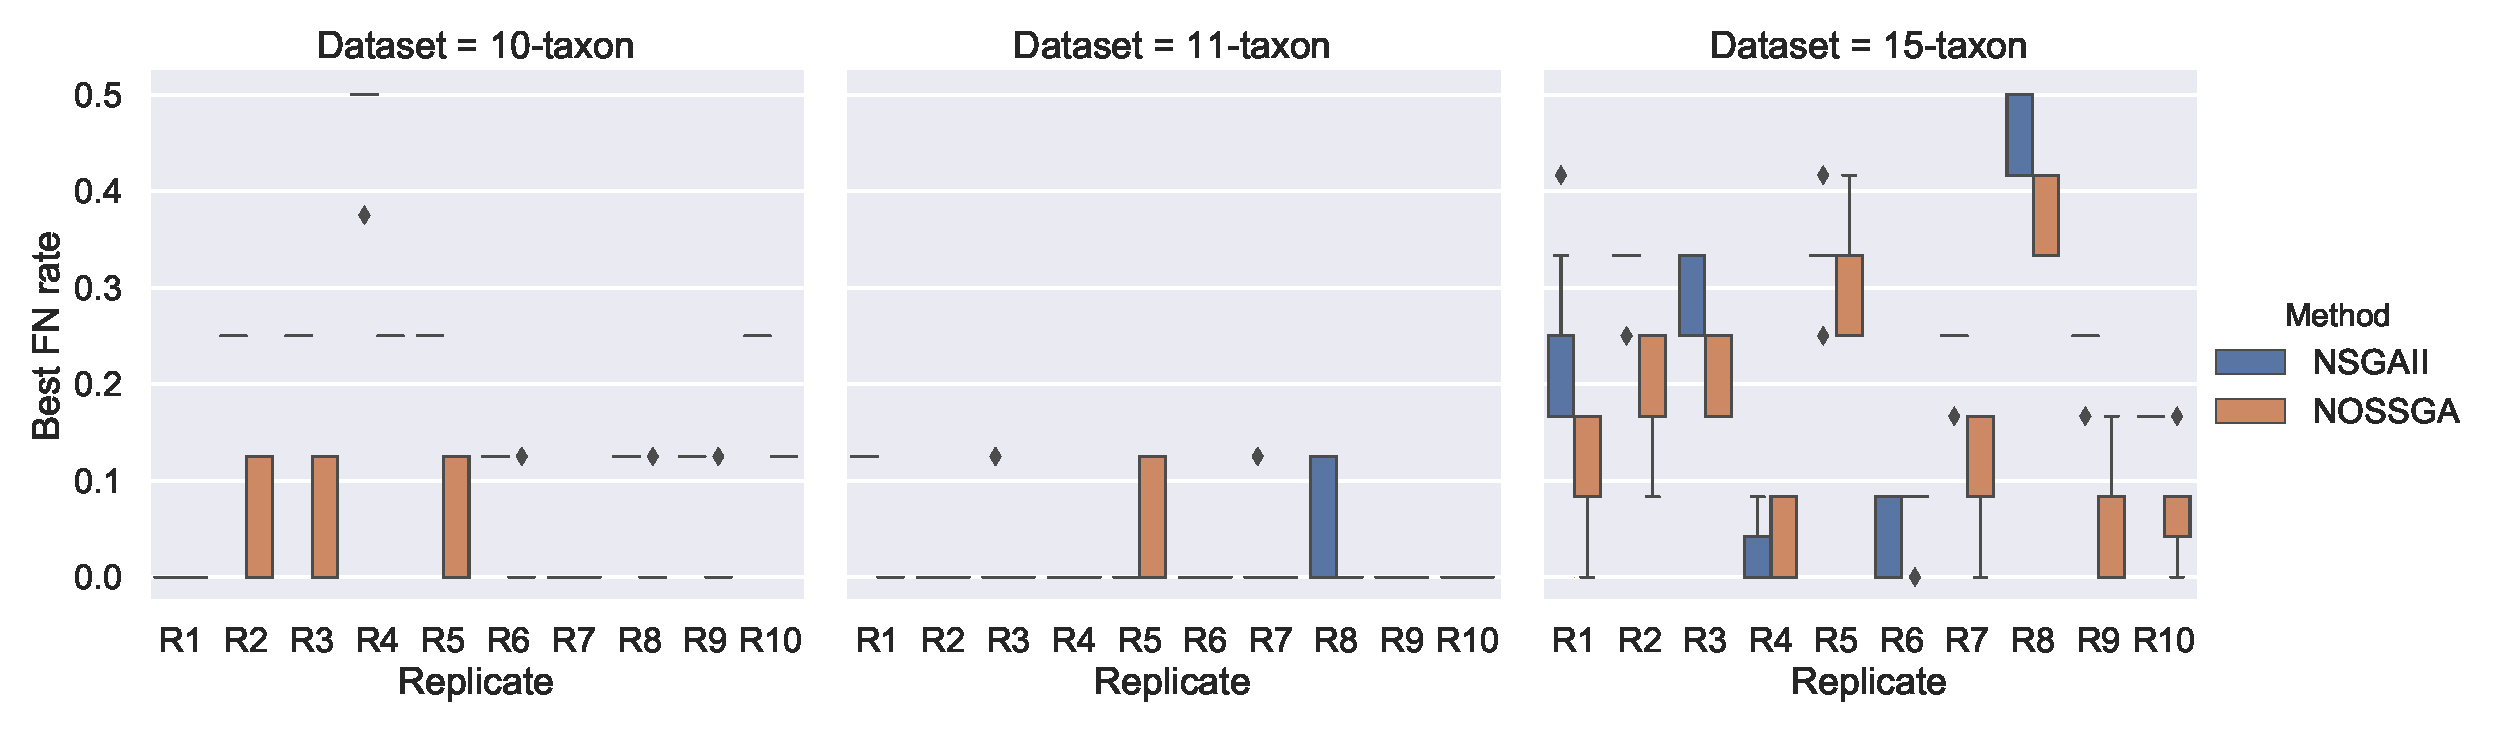
\includegraphics[width=1.5\textwidth]{Figure/emo_boxplot}
		\caption{Accuracy of the best estimated species tree extracted from the final population of NSGAII and NOSSGA on each dataset having 10 replicate.} \label{fig:emo_compare}
	\end{adjustwidth}
\end{figure}
\subsection{Comparison with Existing Methods}
\begin{figure}
	\begin{adjustwidth}{0cm}{0cm}
		\centering
		\includegraphics[width=0.5\textwidth]{Figure/all_dataset_compare}
		\caption{Performance of ASTRAL, STELAR, MP-EST, NSGAII and NOSSGA on three datasets. For each dataset, FN rates are averaged over 10 replicates. We show the average FN rates with standard error bars over 10 replicates} \label{fig:compare_exisitng_methods}
	\end{adjustwidth}
\end{figure}

%\subsection{Discussion}

\begin{comment}
\begin{figure}[!htbp]
	\centering
	\begin{adjustwidth}{-1cm}{}
	\begin{subfigure}[b]{0.55\textwidth}
		\includegraphics[width=\textwidth]{Figure/10-taxon_10_replicates}
		\caption{10-taxon}
		%\label{fig:con_pr06}
	\end{subfigure}%
	\begin{subfigure}[b]{0.55\textwidth}
		\includegraphics[width=\textwidth]{Figure/11-taxon_10_replicates}
		\caption{11-taxon}
		%\label{fig:con_pr07}
	\end{subfigure}%
%	\newline

	\begin{subfigure}[b]{0.55\textwidth}
		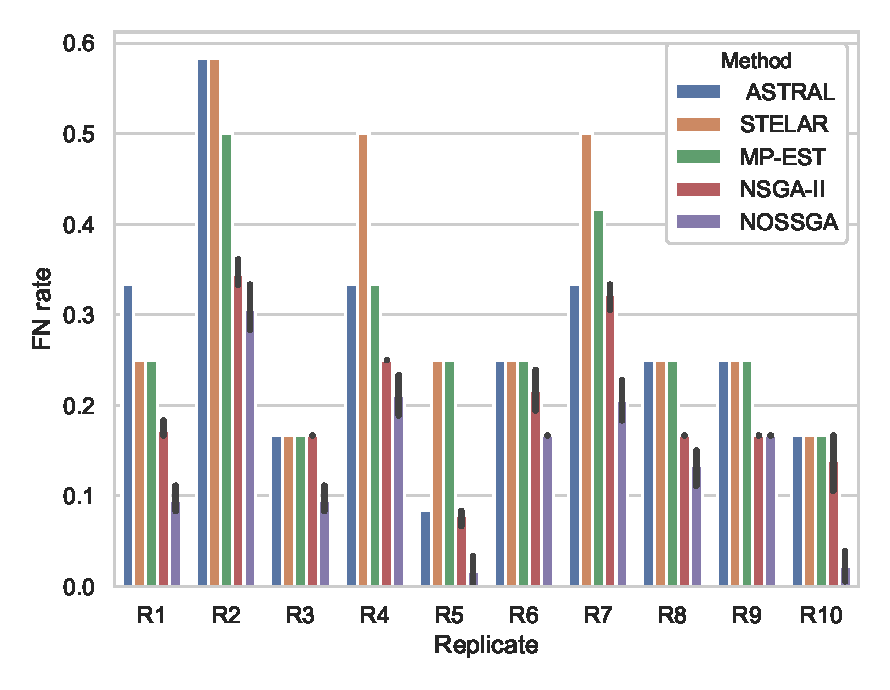
\includegraphics[width=\textwidth]{Figure/15-taxon_10_replicates}
		\caption{15-taxon}
		%\label{fig:con_pr09}
	\end{subfigure}
	\begin{subfigure}[b]{0.55\textwidth}
		\includegraphics[width=\textwidth]{Figure/all_dataset_compare}
		\caption{Summary}
		%\label{fig:con_pr09}
	\end{subfigure}%

	\caption{Comparison of ASTRAL, STELAR, MP-EST, NSGAII and NOSSGA on 10 replicates of 3 datasets.}
	\label{fig:datasets}
\end{adjustwidth}
\end{figure}



\begin{figure}[!htbp]
\centering
\begin{adjustwidth}{-1cm}{}
\begin{subfigure}[b]{0.48\textwidth}
\includegraphics[width=\textwidth]{Figure/10-taxon_NSGA-II_heatmap}
\caption{NSGAII: 10-taxon}
%\label{fig:con_pr06}
\end{subfigure}%
\begin{subfigure}[b]{0.4\textwidth}
\includegraphics[width=\textwidth]{Figure/11-taxon_NSGA-II_heatmap}
\caption{NSGAII: 11-taxon}
%\label{fig:con_pr07}
\end{subfigure}%
\begin{subfigure}[b]{0.4\textwidth}
\includegraphics[width=\textwidth]{Figure/15-taxon_NSGA-II_heatmap}
\caption{NSGAII: 15-taxon}
%\label{fig:con_pr09}
\end{subfigure}

\begin{subfigure}[b]{0.48\textwidth}
\includegraphics[width=\textwidth]{Figure/10-taxon_NOSSGA_heatmap}
\caption{NOSSGA: 10-taxon}
%\label{fig:con_pr06}
\end{subfigure}%
\begin{subfigure}[b]{0.4\textwidth}
\includegraphics[width=\textwidth]{Figure/11-taxon_NOSSGA_heatmap}
\caption{NOSSGA: 11-taxon}
%\label{fig:con_pr07}
\end{subfigure}%
\begin{subfigure}[b]{0.4\textwidth}
\includegraphics[width=\textwidth]{Figure/15-taxon_NOSSGA_heatmap}
\caption{NOSSGA: 15-taxon}
%\label{fig:con_pr09}
\end{subfigure}
\caption{Correlation between each pair of objectives as the generation of an EMO progresses. For each dataset, we average the correlation coefficient over 15 runs and 10 replicates.}
\label{fig:gen_wise_correlation}
\end{adjustwidth}
\end{figure}
%\begin{figure}
%	\centering
%	\includegraphics[width=0.6\textwidth]{Figure/10-taxon_10_replicates}
%	\caption{10-taxon.} \label{fig1}
%\end{figure}
%\begin{figure}
%	\centering
%	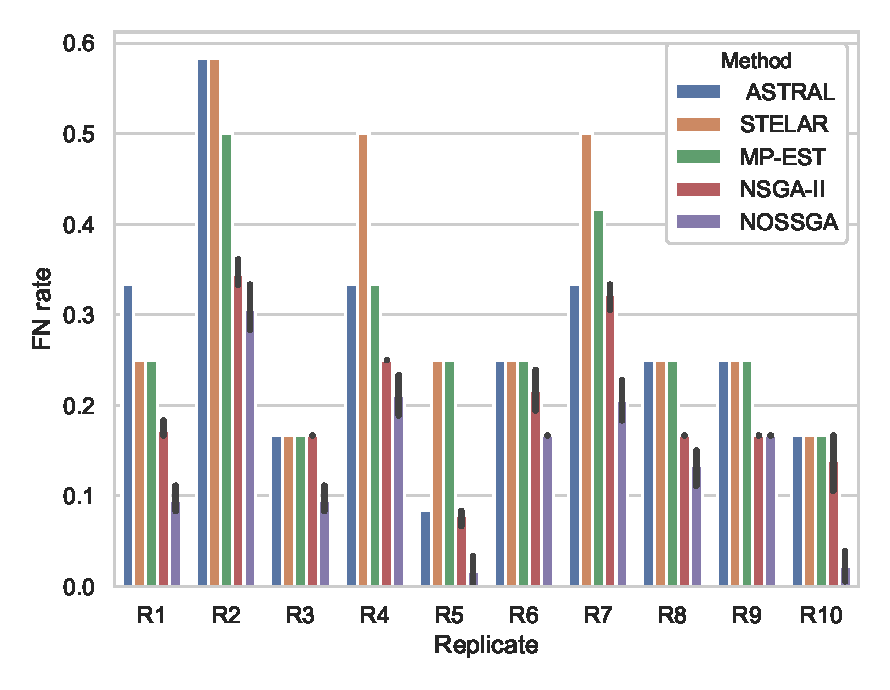
\includegraphics[width=0.6\textwidth]{Figure/15-taxon_10_replicates}
%	\caption{15-taxon.} \label{fig2}
%\end{figure}
\subsection{Results on 10-taxon dataset}
\subsection{Results on 11-taxon dataset}
\subsection{Results on 15-taxon dataset}
\end{comment}

